\chapter{Agujeros Negros ***PRELIMINAR***}


\section{Singularidades y radio de Schwarzschild}

Aquí estudiaremos la estructura de la solución de Schwarzschild en regiones \textit{cercanas al radio de Schwarzschild}, donde el campo gravitacional es muy intenso. En otras palabras, estudiaremos las geometría del espaciotiempo esféricamente simétrico de una masa $M$ suficientemente compacta para que su tamaño (la coordenada radial correspondiente a su superficie) sea menor que $2m$. Por ahora, postergaremos la importante discusión acerca de si existe un mecanismo físico realista para que una distribución de masa pueda llegar a esta configuración.

La geometría del espaciotiempo de Schwarzschild, en coordenadas de
curvatura, es decir (\ref{Sch}), parece tener un mal comportamiento cerca de
$r=0$ y además en $r=2m$, es decir, en el origen y en la esfera definida por
la condición que la coordenada radial $r$ sea igual al radio de Schwarzschild.
\begin{eqnarray}
 g_{00}&\to& -\infty,\quad g_{11}\to 0, \qquad \text{para}\quad r\to 0 ,\\
 g_{00}&\to& 0,\quad g_{11}\to -\infty, \qquad \text{para}\quad r\to 2m^+ .
\end{eqnarray}
Los coeficientes métricos son cantidades dependientes de las coordenadas
usadas, por lo que sus valores no necesariamente están relacionados con
cantidades físicas singulares. Para saber si estos comportamientos
singulares/divergentes son físicos, o sólo \textit{singularidades coordenadas},
necesitamos considerar propiedades que sean independientes de las coordenadas
usadas.

Es relativamente fácil generar singularidades coordenadas. Consideremos por ejemplo, el espacio euclidiano bidimensional $E_2$, con su elemento de línea en coordenadas cartesianas:
\begin{equation}
ds^2=dx^2+dy^2.
\end{equation}
Si introducimos una nueva coordenada $\xi$ por medio de
\begin{equation}
\xi:=\frac{1}{3}x^3,
\end{equation}
tendremos que la métrica toma la forma%
\begin{equation}
ds^2 =\left( 3\xi\right) ^{-\frac{4}{3}}d\xi^2+dy^2.
\end{equation}
La métrica parece tener ahora una singularidad en $\xi=0$. Sin embargo, esta
singularidad es totalmente removible introduciendo una ``nueva"\, variable $x$ por
medio de $\xi=x^3/3$. Por esto, se dice que ésta es una
\textit{singularidad coordenada}. Es posible que tengamos una singularidad coordenada que sea el resultado de un quiebre de un sistema coordenado específico en lugar de ser una singularidad de la variedad subyacente. En otras palabras, se dice que la variedad tiene una singularidad (``verdadera'' o ``intrínseca'') en su geometría \textit{si ella no puede ser removida por un cambio de coordenadas apropiado}. En general no es obvio encontrar la manera de remover una singularidad coordenada.

Una forma de testear si una región contiene singularidades de la geometría (es decir, que no sean simples singularidades coordenadas) es calcular invariantes (es decir, escalares) a partir de contracciones del tensor de curvatura. Los escalares más simples son el escalar de curvatura
$R$, y sus contracciones $R_{\mu\nu\rho\sigma}R^{\mu\nu\rho\sigma}$, $R_{\mu\nu\rho\sigma}R^{\rho\sigma\lambda\tau}R^{\mu\nu}{}_{\lambda\tau}$, etc. Si alguno de estos escalares \textit{diverge} al acercarse a algún punto, tal punto es una singularidad de la geometría. Así, tenemos una condición \textit{suficiente}
para mostrar que un punto es una singularidad de la geometría. Por otro lado, en general no es fácil mostrar que un punto \textit{no es} singularidad.

En el caso de la métrica de Schwarzschild un cálculo directo muestra que
\begin{equation}
R_{\mu\nu\rho\sigma}R^{\mu\nu\rho\sigma}=\frac{48m^2}{r^6},
\end{equation}
lo que prueba que $r=0$ (el origen del sistema coordenado usado) representa una
singularidad de la geometría, donde la curvatura diverge. Puede verificarse que en $r=2m$ ninguno de los invariantes de curvatura arriba mencionados diverge. Por lo tanto, la esfera definida por $r=2m$ no es una singularidad de la curvatura (que mide propiedades locales de la variedad), sino algo diferente ...

\begin{itemize}
\item En $r=2m$, $g_{11}$ es infinito y $g_{00}$ es cero. Dado que $g_{00}
$ es cero, la superficie esférica en $r=2m$ es una \textit{superficie
infinitamente desplazada al rojo} por efecto de la dilatación temporal gravitacional. Ver la expresión (\ref{rgsch}). Decimos entonces que la superficie $r=2m$ es una \textit{superficie de redshift infinito}.

\item Además, cuando $r<2m$, el signo de las componentes $g_{00}$ y $g_{11}$ cambian: $g_{00}$ se convierte en negativo y $g_{11}$ en positivo. Esto nos fuerza a reconsiderar el significado físico de $t$ y $r$. En efecto, en la región del espaciotiempo con $r<2m$, $t$ es una coordenada tipo espacio y $r$ tipo tiempo, ya que una curva a lo largo del eje $t$ ($r$, $\theta$ y $\varphi$ constantes) posee $ds^2<0$, mientras que una curva a lo largo del eje $r$ ($t$, $\theta$ y $\varphi$ constantes) posee $ds^2>0$. Como veremos más adelante, esto trae como consecuencia que toda partícula dentro de la región delimitada por $r=2m$ caerá hacia la singularidad central. Debido a esto, la superficie $r=2m$ es adicionalmente un \textit{horizonte de eventos}.
\end{itemize}

Estas características muestran que $r=2m$ es un radio inusual, pero
esto no implica que la geometría local del espaciotiempo sea
singular en $r=2m$, como sí ocurre en $r=0$.

Para analizar las propiedades físicas de la región en torno a $r=2m$ con más detalle, estudiaremos las propiedades de fotones y de partículas en movimiento radial ``cayendo'' hacia (y ``escapando'' desde) la singularidad central.

\subsection{Diagrama Espacio-Temporal en Coordenadas de Schwarzschild}

Una manera de entender una geometría es explorando su estructura causal, que está definida por las propiedades de propagación de la luz. Consideremos en particular curvas (geodésicas)
radiales tipo luz, es decir, para las cuales $\theta$ y $\varphi$ son constantes y
$ds^2=0$. Esta última condición se reduce a
\begin{equation}
 \left(1-\frac{2m}{r}\right) c^2dt^2-\frac{dr^2}{\left( 1-\frac
{2m}{r}\right) }=0,
\end{equation}
de donde obtenemos que
\begin{equation}
 c\frac{dt}{dr}=\pm\frac{1}{\left| 1-\frac{2m}{r}\right|}. \label{dtdr1}
\end{equation}
Considerando que
\begin{equation}
 \int_a^b\frac{dr}{\left| 1-\frac{2m}{r}\right|}=\pm\left[b-a+2m\ln\left(\frac{b-2m}{a-2m}\right)\right], \quad a<b,
\end{equation}
donde el signo positivo y negativo corresponde a los casos en que $a,b>2m$ y $a,b<2m$, respectivamente, podemos integrar (\ref{dtdr1}).

Si $r>2m$ el signo $+$ en (\ref{dtdr1}) corresponde a fotones alejándose del centro de simetría y el signo $-$ a fotones acercándose a éste. En este caso obtenemos,
\begin{equation}
 c(t-t_0)=r-r_0+2m\ln\left(\frac{r-2m}{r_0-2m}\right),  \label{rtfs}
\end{equation}
para fotones salientes, y
\begin{equation}
 c(t-t_0)=r_0-r-2m\ln\left(\frac{r-2m}{r_0-2m}\right), \label{rtfe}
\end{equation}
para fotones entrantes, que pasan por el evento con coordenadas $(ct_0,r_0)$, respectivamente.
\begin{figure}[H]
 \begin{center}
\includegraphics[height=8cm,angle=-90]{fig/fig-nullrays-cc-01.pdf}
\caption{Curvas nulas radiales en coordenadas de curvatura.}
\label{fig:nullrays-cc}
\end{center}
\end{figure}
Como es de esperar, muy lejos del centro de fuerzas $r\gg 2m$, recobramos
\begin{equation}
\frac{dr}{dt}=\pm\, c,
\end{equation}
tal como en un espaciotiempo plano. Por otro lado, cuando $r$ se aproxima a $2m$ (por ``la derecha'', es decir, con valores mayores a $2m$), tenemos
\begin{equation}
\frac{dt}{dr}\rightarrow\pm\infty,
\end{equation}
y los conos de luz se ``cierran", ya que las líneas tienden a ser
paralelas al eje $t$. Esto tendrá como consecuencia que al acercarse a $r=2m$ la coordenada temporal de la trayectoria del fotón aumentará indefinidamente. En otras palabras, en términos de la coordenada temporal $t$, a medida que un rayo de luz se aproxima a $r=2m$ pareciera que el fotón nunca llegará allí. En realidad, como veremos a continuación, un rayo de luz no tiene problemas en alcanzar $r=2m$ (tampoco partículas masivas), pero un observador lejos de $r=2m$ nunca sería capaz de ``ver'' este hecho.

En efecto, para describir cómo se ``ve''\, la caída del fotón desde lejos, consideraremos un observador en reposo en $r=R>2m$ y cómo éste puede informarse sobre la caída del fotón.

Para esto, consideramos un fotón cayendo hacia la singularidad, y dos eventos $E_1$ y $E_2$ en su línea de mundo, con coordenadas $(ct,r)=(ct_1,r_1)$ y $(ct,r)=(ct_2,r_2)$ respectivamente, con $r_2<r_1<R$. De acuerdo a lo anterior, las coordenadas de estos eventos están relacionadas por medio de
\begin{equation}
c(t_2-t_1)=r_1-r_2+2m\ln\left(\frac{r_1-2m}{r_2-2m}\right). \label{t2t1}
\end{equation}
Consideremos que cuando el fotón pasa por el evento $E_1$ una se~nal luminosa (otro fotón) es enviada hacia el observador en $R>r_1$. Este nuevo fotón viaja desde el evento $E_1$ hasta el evento de recepción $R_1$, con coordenadas $(ct,r)=(ct_{1\rm r},R)$. Como estos eventos pertenecen a la línea de mundo de un fotón alejándose de la singularidad, sus coordenadas satisfacen
\begin{equation}
c(t_{1 \rm r}-t_1)=R-r_1+2m\ln\left(\frac{R-2m}{r_1-2m}\right).\label{t1rt1}
\end{equation}
Similarmente, si en el evento $E_2$ se emite una segunda señal luminosa hasta el observador, de modo que éste la recibe en el evento $R_2$ con coordenadas $(ct,r)=(ct_{2\rm r},R)$, entonces
\begin{equation}
c(t_{2 \rm r}-t_2)=R-r_2+2m\ln\left(\frac{R-2m}{r_2-2m}\right).\label{t2rt2}
\end{equation}
El intervalo de coordenada temporal entre la recepción de las dos se~nales por el observador en reposo en la posición $r=R$ es dada por $(\Delta t)_{\rm r}=t_{2 \rm r}-t_{1 \rm r}$. Usando (\ref{t2t1}), (\ref{t1rt1}) y (\ref{t2rt2}), encontramos
\begin{equation}
c(\Delta t)_{\rm r}=2\left[r_1-r_2+2m\ln\left(\frac{r_1-2m}{r_2-2m}\right)\right].
\end{equation}
En otras palabras, $(\Delta t)_{\rm r}=2(t_2-t_1)$. Finalmente, el tiempo (propio) medido por el observador en $r=R$ entre las dos se~nales es $(\Delta\tau)_{\rm r}=(\Delta t)_{\rm r}\sqrt{1-2m/R}$. En particular, para un observador ``en el infinito", tendremos simplemente que
$(\Delta\tau)_{{\rm r},\infty}=2(t_2-t_1)$. Como consecuencia, desde el punto de vista de un observador externo (en $r=R$, o en el infinito) el fotón requiere un tiempo infinito en llegar a $r=2m$, es decir, \textit{el observador nunca registra que el fotón cruza el horizonte}, sino que lo observa acercarse cada vez más lentamente. No obtante, como veremos a continuación, el fotón no encuentra ningún obstáculo al acercarse al horizonte, cruzándolo y alcanzando finalmente la singularidad central.

\subsection{Coordenadas de Eddington-Finkelstein}

Hemos visto que en términos de las coordenadas de curvatura los conos de luz parecen comprimirse a medida que se acercan a $r=2m$, y que las curvas tipo luz radiales entrantes parecen nunca cruzar el horizonte, ya que estas curvas se tornan cada vez más verticales.

Es posible introducir nuevas coordenadas en las que estas características no están presentes. Específicamente, podemos elegir nuevas coordenadas $\bar{x}^\mu=(c\bar{t},r,\theta,\varphi)$, en las que las líneas nulas radiales entrantes sean rectas con un ángulo de 45 grados respecto al eje $r$. De (\ref{rtfe}) vemos que si definimos la \textit{coordenada de Eddington-Finkelstein retardada} por
\begin{equation}
 \bar{t}(t,r):=t+\frac{2m}{c}\ln\left(r-2m\right), \qquad r>2m, \label{tEF}
\end{equation}
entonces la relación que define la trayectoria de un fotón entrante es simplemente
\begin{equation}
 c(\bar{t}-\bar{t}_0)=r_0-r,
\end{equation}
que en el plano $(c\bar{t},r)$  corresponde precisamente una línea recta con pendiente $-1$.

En términos de las nuevas coordenadas $\bar{x}^\mu$ el elemento de línea adopta la forma siguiente:
\begin{equation}\marginnote{Schwarzschild, Eddington-Finkelstein}
 ds^2=\left(1-\frac{2m}{r}\right)c^2d\bar{t}^2-\frac{4m}{r}c\,d\bar{t}\,dr-\left(1+\frac{2m}{r}\right)dr^2-r^2\left(d\theta^2+\sen^2\theta\,d\varphi^2\right). \label{dsEF}
\end{equation}
Vemos que la métrica en estas coordenadas es regular en $r=2m$. De hecho, ella es regular en todo el rango $0<r<2m$. Puede argumentarse que la transformación (\ref{tEF}) no es válida para puntos con $r\le 2m$ y que por consiguiente (\ref{dsEF}) sólo sería válida en la región fuera del horizonte. Sin embargo, en la teoría de RG, el criterio usado es que, dada una métrica que es solución de las Ecuaciones de Einstein, se busca el rango máximo de variación de las coordenadas tales que la solución sea analítica (libre de divergencias). En otras palabras, puede perfectamente considerarse la métrica en coordenadas de Eddington-Finkelstein como la ``métrica original'', válida en todo el rango $0<r<\infty$, y la métrica en coordenadas de curvatura como sólo apropiada en la región exterior al horizonte. En cierto sentido, la métrica en coordenadas Eddington-Finkelstein es una suerte de ``continuación analítica'' de la métrica de la solución en coordenadas de curvatura.

Como vimos, en coordenadas de Eddington-Finkelstein, las líneas nulas radiales entrantes son líneas rectas. Por otro lado, las curvas nulas radiales \textit{salientes} están descritas por la relación
\begin{equation}
 c(\bar{t}-\bar{t}_0)=r-r_0+4m\ln\left|\frac{r-2m}{r_0-2m}\right|,  \label{rtfsEF}
\end{equation}
que se obtiene directamente de (\ref{rtfs}) y la definición (\ref{tEF}).

\begin{figure}[H]
 \begin{center}
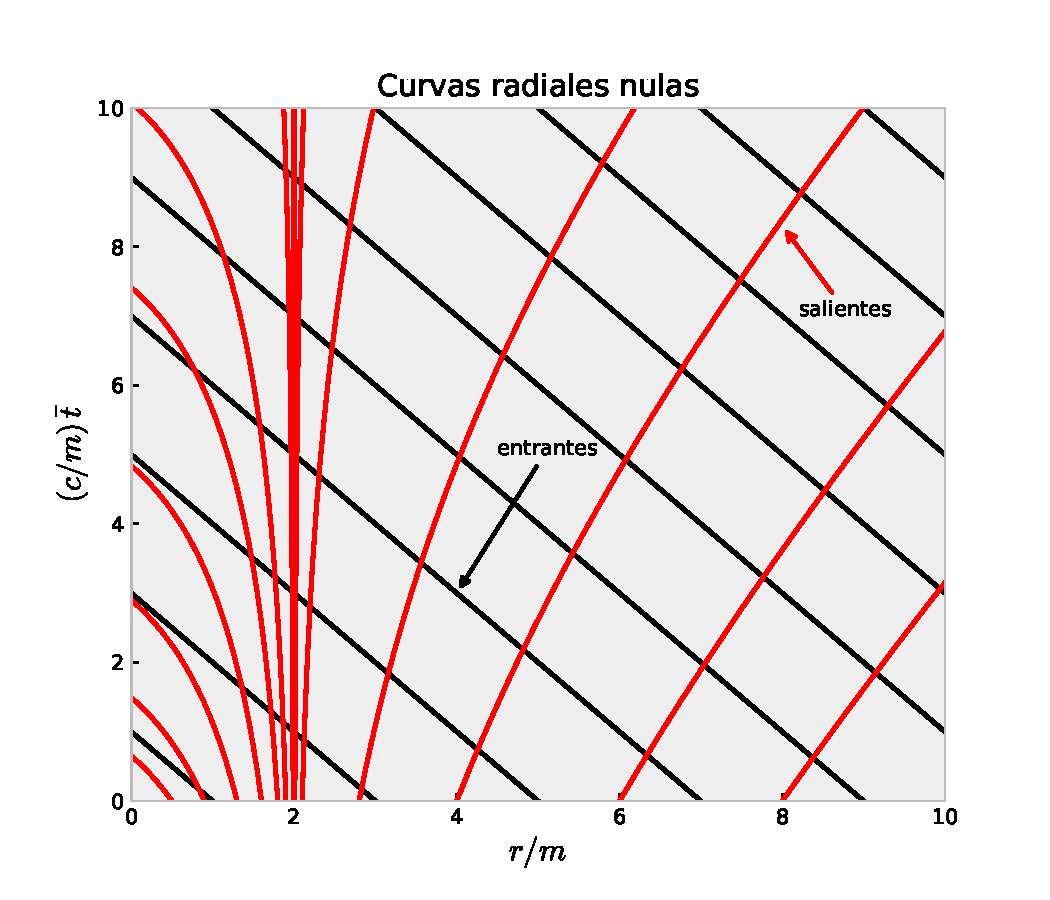
\includegraphics[height=6cm]{fig/fig-nullrays-cEF.pdf}
\caption{Curvas nulas radiales en coordenadas de Eddington-Finkelstein retardadas.}
\label{fig:nullrays-cEF}
\end{center}
\end{figure}

Vemos que la superficie definida por $r=2m$ actúa como una ``membrana unidireccional'', en el sentido que sólo permite cruzar a partículas cayendo hacia la singularidad central. Las líneas de mundo entrantes cruzan desde la región externa hacia la interna. La superficie $r=2m$ es llamada un \textit{horizonte de eventos} ya que representa la región que delimita los eventos que pueden ser en principio observados por un observador externo. El horizonte de Schwarzschild es \textit{absoluto} en el sentido que impide \textit{a todo observador externo} obtener información de eventos dentro del horizonte.

\subsection{Partículas cayendo radialmente}

Consideremos la trayectoria de una partícula cayendo libremente en un movimiento radial hacia la singularidad. La trayectoria es entonces una geodésica radial tipo tiempo. De acuerdo a lo estudiado anteriormente, en este caso la trayectoria tiene como constantes de movimiento a $k$ y $h$ dadas por (\ref{kh}), con $h=0$. De entre las posibles trayectorias, deteminadas por la constante $k$, nos concentraremos en aquellas correspondientes a partículas que caen  ``desde el reposo en el infinito'', es decir, tal que $\dot{r}\to 0$ para $r\to\infty$. En este caso la relación (\ref{uuc22}) implica que $k^2=1$. Finalmente, (\ref{kh}a), muestra que para trayectorias ``orientadas hacia el futuro'', $k=1$. Con esto, (\ref{uuc22}) se reduce en este caso a
\begin{equation}
\dot{r}^2 =\frac{2mc^2}{r} .\label{pi1}
\end{equation}
Como estamos considerando una partícula acercándose a la singularidad central, tendremos entonces que
\begin{equation}
\frac{dr}{d\tau}=-c\sqrt{\frac{2m}{r}} .
\end{equation}
Podemos integrar esta expresión directamente, y obtenemos
\begin{equation}
 c(\tau-\tau_0)=\frac{2}{3\sqrt{2m}}\left(r_0^{3/2}-r^{3/2}\right), \label{taurclr}
\end{equation}
donde $\tau_0$ es el tiempo propio (del reloj comóvil con la partícula) registrado en el instante en que ésta pasa por $r=r_0$. Note que la expresión encontrada, (\ref{taurclr}), es la misma que el caso newtoniano. Como consecuencia, el intervalo de tiempo propio desde que la partícula cruza $r=r_0$ y que llega a la singularidad central es finito:
\begin{equation}
 c(\tau|_{r=0}-\tau_0)=\frac{2}{3\sqrt{2m}}r_0^{3/2}.
\end{equation}
En particular, el tiempo propio requerido para caer desde el horizonte hasta la singularidad central es $4m/3c$

Para analizar cómo varía la coordenada $t$ en este proceso, podemos escribir
\begin{equation}
 c\frac{dt}{dr}=c\frac{\dot{t}}{\dot{r}}=-\frac{1}{1-\frac{2m}{r}}\sqrt{\frac{r}{2m}}.
\end{equation}
Integrando esta expresión\footnote{$\int\sqrt{\frac{r}{a}}\frac{dr}{1-\frac{a}{r}}=\frac{2}{3}a\, (r/a)^{3/2}+2a\,(r/a)^{1/2}-a\ln\left(\frac{\sqrt{r}-\sqrt{a}}{\sqrt{r}+\sqrt{a}}\right) $.} encontramos
\begin{equation}
c(t-t_0)=-\frac{2}{3\sqrt{2m}}\left(r^{3/2} -r_0^{3/2}+6m\sqrt{r}-6m\sqrt{r_0}\right)+2m\ln\left[\frac{(\sqrt{r}+\sqrt{2m})(\sqrt{r_0}-\sqrt{2m})}{(\sqrt{r}-\sqrt{2m})(\sqrt{r_0}+\sqrt{2m})}\right].
\end{equation}
Vemos de esta expresión que la coordenada temporal de la trayectoria de la partícula crece indefinidamente a medida que ésta se acerca al horizonte.

% \section{Coordenadas de Eddington-Finkelstein}
%
% \begin{align}
% \left[ \left( 1-\frac{2m}{r}\right) \frac{2m^2}{\left(
% r-2m\right) ^2}-\frac{1}{\left( 1-\frac{2m}{r}\right) }\right]
% dr^2 & =\left[ \frac{2m^2}{r\left( r-2m\right) }-\frac
% {1}{\left( 1-\frac{2m}{r}\right) }\right] dr^2\\
% & =\left[ \frac{\left( 1-\frac{2m}{r}\right) 2m^2-r\left(
% r-2m\right) }{r\left( r-2m\right) \left( 1-\frac{2m}{r}\right)
% }\right] dr^2\\
% & =\left[ \frac{2m^2-r^2}{r\left( r-2m\right) }\right] dr^2\\
% & =\left[ \frac{\left( 2m-r\right) \left( 2m+r\right) }{r\left(
% r-2m\right) }\right] dr^2\\
% & =-\left[ \frac{\left( r-2m\right) \left( 2m+r\right) }{r\left(
% r-2m\right) }\right] dr^2\\
% & =-\left[ \frac{\left( 2m+r\right) }{r}\right] dr^2=-\left[
% 1+\frac{2m}{r}\right] dr^2%
% \end{align}
% de manera que%
% \begin{equation}
% ds^2=\left( 1-\frac{2m}{r}\right) d\overline{t}^2-\frac{22m}%
% {r}d\overline{t}dr-\left( 1+\frac{2m}{r}\right) dr^2-r^2d\Omega
% ^2\label{ef9}%
% \end{equation}
% expresión conocida como la forma de Eddington-Finkelstein de la
% métrica de Schwarzchild. Notemos que la solución es ahora regular en
% $r=2m$, además es también regular para todo el rango $\left(
% 0<r<2m\right) $. De modo que en algún sentido, la transformación
% dada por la Ec. (\ref{ef6}) extiende el rango de las
% coordenadas desde $2m<r<\infty$ a $0<r<\infty$. El proceso es alguna
% reminiscencia de una continiación analítica de una función en
% análisis complejo. Debido a esto Ec. (\ref{ef9}) es llamada
% la extensión analítica de la solución de Schwarzschild.
% Podría ser objetado que la transformación de coordenadas dada por
% Ec. (\ref{ef5}) no puede ser usada en $r=2m$ debido a que
% ella se convierte en singular. Sin embargo, Ec. (\ref{ef5}) es
% una herramienta conveniente para ir desde la solución de Schwarzschild a
% Ec. (\ref{ef9}). Nuestro punto de partida es en realidad en
% base a estos dos elementos de línea. Dadas estas soluciones, la pregunta
% es \textquestiondown Cuál es el mayor rango de las coordenadas para las
% cuales cada solución es regular?. La respuesta es $2m<r<\infty$ para la
% solución de Schwarzschild y $0<r<\infty$ para la forma de
% Eddington-Finkelstein (junto, obviamente a $-\infty<t<\infty,$ $0\leq
% \theta\leq\pi$ y $-\pi\leq\varphi\leq\pi$). En la región de traslape
% ($2m<r<\infty$), las dos soluciones están relacionadas por medio de la
% transformación \ref{ef5} y por lo tanto, ellas representan la misma
% solución en esta región.
%
% Notemos que la solución en las coordenadas de Eddington-Finkelstein no es
% simétrica en el tiempo. Podemos obtener una solución con el tiempo
% inverso introduciendo, en lugar de Ec. (\ref{ef6}), la
% siguiente transformación en la coordenada temporal%
% \begin{equation}
% t\rightarrow\overline{t}=t-2m\ln\left( \frac{2m}{r}-1\right)
% \label{ef10}%
% \end{equation}
% para $r>2m$. Esto implica que la congruencia \ref{ef4} toma la forma
% \begin{align}
% t & =r+2m\ln\left( \frac{r}{2m}-1\right) +cte\nonumber\\
% \overline{t}+2m\ln\left( \frac{2m}{r}-1\right)  & =r+2m\ln\left(
% \frac{r}{2m}-1\right) +cte\nonumber\\
% \overline{t} & =r+cte\label{ef11}%
% \end{align}
% la cual es una línea que forma un ángulo de $45^{\circ}$ con el eje
% $r$. De Ec. (\ref{ef10}) vemos que
% \begin{equation}
% d\overline{t}=dt-2m\frac{1}{\frac{r}{2m}-1}d\left( \frac{r}{2m%
% }\right) =dt-\frac{1}{\frac{r-2m}{2m}}dr=dt-\frac{2m}{r-2m}dr
% \end{equation}
% $\Longrightarrow$%
% \begin{equation}
% dt=d\overline{t}+\frac{2m}{r-2m}dr\label{ef12}%
% \end{equation}
%
%
% Introduciendo Ec. (\ref{ef12}) en la solución de Schwarzschild tenemos%
% \begin{align}
% ds^2 & =\left( 1-\frac{2m}{r}\right) dt^2-\frac{dr^2}{\left(
% 1-\frac{2m}{r}\right) }-r^2d\Omega^2\nonumber\\
% ds^2 & =\left( 1-\frac{2m}{r}\right) \left( d\overline{t}+\frac
% {2m}{r-2m}dr\right) ^2-\frac{dr^2}{\left( 1-\frac{2m}%
% {r}\right) }-r^2d\Omega^2\nonumber\\
% ds^2 & =\left( 1-\frac{2m}{r}\right) \left( d\overline{t}^2%
% +2\frac{2m}{r-2m}d\overline{t}dr+\frac{2m^2}{\left( r-2m%
% \right) ^2}dr^2\right) -\frac{dr^2}{\left( 1-\frac{2m}{r}\right)
% }-r^2d\Omega^2\nonumber\\
% ds^2 & =\left( 1-\frac{2m}{r}\right) \left( d\overline{t}^2%
% +2\frac{2m}{r-2m}d\overline{t}dr+\frac{2m^2}{\left( r-2m%
% \right) ^2}dr^2\right) -\frac{dr^2}{\left( 1-\frac{2m}{r}\right)
% }-r^2d\Omega^2\nonumber\\
% ds^2 & =\left( 1-\frac{2m}{r}\right) d\overline{t}^2+2\left(
% 1-\frac{2m}{r}\right) \frac{2m}{r-2m}d\overline{t}dr+\left(
% 1-\frac{2m}{r}\right) \frac{2m^2}{\left( r-2m\right) ^2}%
% dr^2-\frac{dr^2}{\left( 1-\frac{2m}{r}\right) }-r^2d\Omega
% ^2\nonumber\\
% ds^2 & =\left( 1-\frac{2m}{r}\right) d\overline{t}^2+2\left(
% \frac{r-2m}{r}\right) \frac{2m}{r-2m}d\overline{t}dr+\left(
% \frac{r-2m}{r}\right) \frac{2m^2}{\left( r-2m\right) ^2}%
% dr^2-\frac{rdr^2}{\left( r-2m\right) }-r^2d\Omega^2\nonumber\\
% ds^2 & =\left( 1-\frac{2m}{r}\right) d\overline{t}^2+2\frac{2m%
% }{r}d\overline{t}dr+\left[ \left( \frac{r-2m}{r}\right) \frac{2m^2%
% }{\left( r-2m\right) ^2}-\frac{r}{\left( r-2m\right) }\right]
% dr^2-r^2d\Omega^2\nonumber\\
% ds^2 & =\left( 1-\frac{2m}{r}\right) d\overline{t}^2+2\frac{2m%
% }{r}d\overline{t}dr+\left[ \frac{2m^2}{r\left( r-2m\right) }%
% -\frac{r}{\left( r-2m\right) }\right] dr^2-r^2d\Omega^2\nonumber\\
% ds^2 & =\left( 1-\frac{2m}{r}\right) d\overline{t}^2+2\frac{2m%
% }{r}d\overline{t}dr+\left[ \frac{2m^2-r^2}{r\left( r-2m\right)
% }\right] dr^2-r^2d\Omega^2\nonumber\\
% ds^2 & =\left( 1-\frac{2m}{r}\right) d\overline{t}^2+2\frac{2m%
% }{r}d\overline{t}dr+\left[ \frac{\left( 2m-r\right) \left(
% 2m+r\right) }{r\left( r-2m\right) }\right] dr^2-r^2d\Omega
% ^2\nonumber\\
% ds^2 & =\left( 1-\frac{2m}{r}\right) d\overline{t}^2+2\frac{2m%
% }{r}d\overline{t}dr-\left( 1+\frac{2m}{r}\right) dr^2-r^2d\Omega
% ^2\label{ef13}%
% \end{align}
% expresión conocida como la métrica de Schwarzchild en coordenadas de
% Eddington-Finkelstein. Así, la expresión más general para la
% métrica de Schwarzschild en las coordenadas de Eddington-Finkelstein viene
% dada por%
% \begin{equation}
% ds^2=\left( 1-\frac{2m}{r}\right) d\overline{t}^2\pm2\frac{2m}%
% {r}d\overline{t}dr-\left( 1+\frac{2m}{r}\right) dr^2-r^2d\Omega
% ^2\label{ef14}%
% \end{equation}
% Esta forma de la métrica es de nuevo independiente del tiempo pero no es
% diagonal. La métrica es ahora no singular en $r=2m$ y satisface las
% ecuaciones de campo de Einstein para todo valor $r>0$. Notemos sin embargo,
% que es requerida una transformación singular para obtener este resultado.
%
% Mostremos ahora que las regiones a ambos lados de la superficie $r=2m$ se
% unen en forma suave sobre esta superficie. Un detallado entendimiento de la
% situación se obtiene examinando la estructura general de los conos de luz
% de la métrica dada por Ec. (\ref{ef14}) en el plano
% $\left( \overline{t},r\right) $. Consideremos primero el caso del signo
% $\left( -\right) $.\ En este caso las direcciones radiales nulas ,con
% $\theta$ y $\varphi$ constantes, serán determinadas por la ecuación%
% \begin{align}
% & ds^2=\left( 1-\frac{2m}{r}\right) d\overline{t}^2-2\frac{2m}%
% {r}d\overline{t}dr-\left( 1+\frac{2m}{r}\right) dr^2=0\nonumber\\
% & d\overline{t}^2-\frac{2m}{r}d\overline{t}^2-2\frac{2m}%
% {r}d\overline{t}dr-dr^2+\frac{2m}{r}dr^2=0\nonumber\\
% & d\overline{t}^2-dr^2-\frac{2m}{r}\left( d\overline{t}^2%
% +2d\overline{t}dr+dr^2\right) =0\nonumber\\
% & d\overline{t}^2-dr^2-\frac{2m}{r}\left( d\overline{t}+dr\right)
% ^2=0\nonumber\\
% & \left( d\overline{t}-dr\right) \left( d\overline{t}+dr\right)
% -\frac{2m}{r}\left( d\overline{t}+dr\right) ^2=0\nonumber\\
% & \left( d\overline{t}+dr\right) \left[ \left( d\overline{t}-dr\right)
% -\frac{2m}{r}\left( d\overline{t}+dr\right) \right] =0\nonumber\\
% & \left( d\overline{t}+dr\right) \left[ d\overline{t}-dr-\frac{2m}%
% {r}d\overline{t}-\frac{2m}{r}dr\right] =0\nonumber\\
% & \left( d\overline{t}+dr\right) \left[ \left( 1-\frac{2m}{r}\right)
% d\overline{t}-\left( 1+\frac{2m}{r}\right) dr\right] =0\label{ef15}%
% \end{align}
% de donde vemos que las direcciones nulas vienen dadas por%
% \begin{align}
% d\overline{t}+dr & =0\Longrightarrow\frac{dr}{d\overline{t}}=-1\label{ef16}\\
% \left( 1-\frac{2m}{r}\right) d\overline{t}-\left( 1+\frac{2m}%
% {r}\right) dr & =0\Longrightarrow\frac{dr}{d\overline{t}}=\frac{r-2m%
% }{r+2m}\label{ef17}%
% \end{align}
%
%
% Las líneas que son tangentes a una u otra de las direcciones dadas por
% Ec. (\ref{ef16}), (\ref{ef17}) son geodésicas radiales nulas.
% De Ec. (\ref{ef16}) vemos que la primera familia de geodésicas nulas posee la
% ecuación%
% \begin{equation}
% d\left( \overline{t}+r\right) =0\Longrightarrow\overline{t}%
% +r=cte\label{ef18}%
% \end{equation}
% estas son líneas geodésicas paralelas. La Ec. (\ref{ef17}) posee una
% integral menos simple. De ella vemos que
% \begin{align}
% \frac{dr}{d\overline{t}} & \rightarrow1\text{ para }r\rightarrow\infty\\
% \frac{dr}{d\overline{t}} & \rightarrow-1\text{ para }r\rightarrow0\\
% \frac{dr}{d\overline{t}} & \rightarrow0\text{ para }r\rightarrow 2m%
% \end{align}
%
%
% De la tercera de estas propiedades vemos que estas geodésicas no cruzan la
% superficie $r=2m$ y serán de la forma mostrada en la figura.
%
% Es de interés recordar que las partículas se mueven sobre líneas
% de universo tipo tiempo o sobre líneas de universo nulas, es decir, sobre
% líneas que yacen en el interior o en la superficie del cono de luz. De la
% figura vemos que para $r>2m$ ninguna partícula puede atravesar la
% hipersfera $r=2m$. Además cualquier partícula que en algún
% momento está en el interior de la superficie $r=2m$, se moverá
% necesariamente hacia $r=0$ alcanzando esta línea en un tiempo finito, sea
% este coordenado o propio.
%
% El hecho de que ninguna partícula, que en algún momento está en
% el interior de la superficie, pueda atravesar la superficie $r=2m$,
% significa que un observador $P$ situado en la región $r>2m$ no puede
% recibir ninguna información acerca de eventos que ocurren al interior de
% la superficie $r=r_{0.}$ Por esto decimos que la hipersuperficie $r=2m$ es
% un horizonte de eventos para todos los observadores ubicados en la región
% \thinspace$r>2m.$
%
% Consideremos ahora el caso del signo $\left( +\right) $. Las direcciones
% radiales nulas manteniendo $\theta,\varphi$ constantes son determinadas por
% \begin{align}
% & ds^2=\left( 1-\frac{2m}{r}\right) d\overline{t}^2+2\frac{2m}%
% {r}d\overline{t}dr-\left( 1+\frac{2m}{r}\right) dr^2=0\\
% & d\overline{t}^2-\frac{2m}{r}d\overline{t}^2+2\frac{2m}%
% {r}d\overline{t}dr-dr^2-\frac{2m}{r}dr^2=0\\
% & d\overline{t}^2-dr^2-\frac{2m}{r}\left( d\overline{t}^2%
% -2d\overline{t}dr+dr^2\right) =0\\
% & \left( d\overline{t}-dr\right) \left( d\overline{t}+dr\right)
% -\frac{2m}{r}\left( d\overline{t}-dr\right) ^2=0\\
% & \left( d\overline{t}-dr\right) \left[ \left( d\overline{t}+dr\right)
% -\frac{2m}{r}\left( d\overline{t}-dr\right) \right] =0\\
% & \left( d\overline{t}-dr\right) \left[ \left( 1-\frac{2m}{r}\right)
% d\overline{t}+\left( 1+\frac{2m}{r}\right) dr\right] =0
% \end{align}
% de donde vamos que las direcciones radiales nulas vienen dadas por%
% \begin{equation}
% d\overline{t}-dr=0\Longrightarrow\frac{dr}{d\overline{t}}=1\Longrightarrow
% \overline{t}-r=cte
% \end{equation}
% las cuales son rectas paralelas que forman un ángulo de $45^{\circ}$ con
% el eje $r$. De aqui vemos que las partículas no tienen problemas para
% "salir" desde $r=0$ y atravesar la hipersuperficie $r=2m$. Por otra parte%
% \begin{align}
% & \left( 1-\frac{2m}{r}\right) d\overline{t}+\left( 1+\frac{2m}%
% {r}\right) dr=0\\
% & \frac{dr}{d\overline{t}}=-\frac{\left( 1-\frac{2m}{r}\right) }{\left(
% 1+\frac{2m}{r}\right) }\\
% & \frac{dr}{d\overline{t}}=-\frac{\left( r-2m\right) }{\left(
% r+2m\right) }%
% \end{align}
% de donde vemos que esta segunda familia tiene las siguientes propiedades:%
%
% \begin{align}
% \frac{dr}{d\overline{t}} & \rightarrow-1\ \text{\ para }%
% r\rightarrow\infty\nonumber\\
% \frac{dr}{d\overline{t}} & \rightarrow1\ \text{\ para }%
% r\rightarrow0\nonumber\\
% \frac{dr}{d\overline{t}} & \rightarrow0\text{ \ para }r\rightarrow
% 2m\label{efx1}%
% \end{align}
% al igual que en el caso anterior, ec. (\ref{efx1}) indica que
% estas familias de goedésicas nulas nunca atraviesan la superficie
% $r=2m$ y al contrario del caso anterior, cualquier partícula que se
% mueva al interior de $r=2m$, se moverá asintóticamente hacia
% $r=2m$ y nunca tocará la singularidad $r=0.$Para un observador ubicado
% en la región $r>2m$ vemos que este también se mueve
% asintóticamente a la hipersuperficie $r=2m$. De esta forma vemos que
% los eventos en las regiones $r>2m$ y $r<2m$ están desconectados, por
% lo tanto, $r=2m$ sigue siendo un horizonte de eventos.




% \section{Coordenadas de Kruskal}
%
% Kruskal introdujo un sistema coordenado esféricamente simétrico en el
% cual los rayos de luz radial tienen en todas partes la pendiente $\frac
% {dr}{dt}=\pm1$. Consideremos la solución a la ecuación
% \begin{equation}
% \frac{dt}{dr}=\pm\left( 1-\frac{2m}{r}\right) ^{-1}%
% \end{equation}
% la cual es dada por%
% \begin{equation}
% t=\pm r^{\ast}+cte=\pm\left[ r+2m\ln\left( \frac{r}{2m}-1\right)
% \right] +cte
% \end{equation}
% las coordenadas de Eddington-Finkelstein se obtienen haciendo%
% \begin{equation}
% t\rightarrow\overline{t}_{\pm}=t\pm 2m\ln\left( \frac{2m}{r}-1\right)
% \text{, para }r>2m%
% \end{equation}
% en las cuales%
% \begin{equation}
% ds^2=\left( 1-\frac{2m}{r}\right) d\overline{t}_{\pm}^2\pm
% 2\frac{2m}{r}d\overline{t_{\pm}}dr-\left( 1+\frac{2m}{r}\right)
% dr^2-r^2d\Omega^2\label{ck1}%
% \end{equation}
% la Ec. (\ref{ck1}) puede ser escrita de una manera más simple introduciendo
% una coordenada nula
% \begin{equation}
% v=\overline{t}_{+}+r\label{ck2}%
% \end{equation}
% conocida como \textit{parámetro de tiempo avanzado}$.$%
% \begin{align}
% dv & =d\overline{t}_{+}+dr\\
% d\overline{t}_{+} & =dv-dr\\
% d\overline{t}_{+}^2 & =dv^2-2dvdr+dr^2%
% \end{align}
% $\Longrightarrow$%
% \begin{align}
% ds^2 & =\left( 1-\frac{2m}{r}\right) d\overline{t_{+}}^2%
% -2\frac{2m}{r}d\overline{t_{+}}dr-\left( 1+\frac{2m}{r}\right)
% dr^2-r^2d\Omega^2\nonumber\\
% ds^2 & =\left( 1-\frac{2m}{r}\right) \left( dv^2-2dvdr+dr^2%
% \right) -2\frac{2m}{r}\left( dv-dr\right) dr-\left( 1+\frac{2m}%
% {r}\right) dr^2-r^2d\Omega^2\nonumber\\
% ds^2 & =\left( 1-\frac{2m}{r}\right) dv^2-2\left( 1-\frac{2m}%
% {r}\right) dvdr+\left( 1-\frac{2m}{r}\right) dr^2\nonumber\\
% & -2\frac{2m}{r}dvdr+2\frac{2m}{r}dr^2-\left( 1+\frac{2m}%
% {r}\right) dr^2-r^2d\Omega^2\nonumber\\
% ds^2 & =\left( 1-\frac{2m}{r}\right) dv^2-2dvdr+2\frac{2m}%
% {r}dvdr+\left( 1-\frac{2m}{r}\right) dr^2\nonumber\\
% & -2\frac{2m}{r}dvdr+2\frac{2m}{r}dr^2-\left( 1+\frac{2m}%
% {r}\right) dr^2-r^2d\Omega^2\nonumber\\
% ds^2 & =\left( 1-\frac{2m}{r}\right) dv^2-2dvdr+\left(
% 1-\frac{2m}{r}\right) dr^2+2\frac{2m}{r}dr^2-\left( 1+\frac{2m%
% }{r}\right) dr^2-r^2d\Omega^2\nonumber\\
% ds^2 & =\left( 1-\frac{2m}{r}\right) dv^2-2dvdr+dr^2-\frac{2m%
% }{r}dr^2+2\frac{2m}{r}dr^2-dr^2-\frac{2m}{r}dr^2-r^2%
% d\Omega^2\nonumber\\
% ds^2 & =\left( 1-\frac{2m}{r}\right) dv^2-2dvdr-r^2d\Omega
% ^2\label{ck3}%
% \end{align}
% si en lugar de Ec. (\ref{ck2}) usamos la coordenada nula%
% \begin{equation}
% w=\overline{t_{-}}+r\text{ , con }\overline{t_{-}}=t-2m\ln\left( \frac
% {r}{2m}-1\right)
% \end{equation}
% conocido como \textit{parámetro temporal retardado} se tiene%
% \begin{equation}
% ds^2=\left( 1-\frac{2m}{r}\right) dw^2+2dwdr-r^2d\Omega
% ^2\label{ck4}%
% \end{equation}
%
%
% Consideremos ahora las coordenadas nulas introducidas de la forma%
% \begin{align}
% v-w & =\overline{t_{+}}+r-\left( \overline{t_{-}}-r\right) =2r+\overline
% {t_{+}}-\overline{t_{-}}\\
% v+w & =\overline{t_{+}}+r+\left( \overline{t_{-}}-r\right) =\overline
% {t_{+}}-\overline{t_{-}}%
% \end{align}
% $\Longrightarrow$%
% \begin{align}
% v-w & =2r+t+2m\ln\left( \frac{r}{2m}-1\right) -\left( t-2m%
% \ln\left( \frac{r}{2m}-1\right) \right) \\
% & =2r+t+2m\ln\left( \frac{r}{2m}-1\right) -t+2m\ln\left( \frac
% {r}{2m}-1\right) \\
% & =2r+22m\ln\left( \frac{r}{2m}-1\right)
% \end{align}
% y%
% \begin{align}
% v+w & =t+2m\ln\left( \frac{r}{2m}-1\right) +t-2m\ln\left(
% \frac{r}{2m}-1\right) \\
% & =2t
% \end{align}
% demodo que podemos introducir las coordenadas $v$ y $w$ por medio de%
% \begin{align}
% v-w & =2\left\{ r+2m\ln\left( \frac{r}{2m}-1\right) \right\}
% =2r^{\ast}\Longrightarrow\frac{1}2\left( v-w\right) =r^{\ast}\\
% v+w & =2t\Longrightarrow\frac{1}2\left( v+w\right) =t
% \end{align}
% dado que
% \begin{equation}
% dr^2=\left( 1-\frac{2m}{r}\right) ^2\left( dr^{\ast}\right) ^2%
% \end{equation}
% y que%
% \begin{align}
% dr^{\ast} & =\frac{1}2\left( dv-dw\right) \\
% dr^{\ast2} & =\frac{1}{4}\left( dv-dw\right) ^2%
% \end{align}
% tenemos%
% \begin{align}
% dr^2 & =\frac{1}{4}\left( 1-\frac{2m}{r}\right) ^2\left(
% dv-dw\right) ^2\\
% & =\frac{1}{4}\left( 1-\frac{2m}{r}\right) ^2\left( dv^2%
% -2dvdw+dw^2\right) \\
% dt^2 & =\frac{1}{4}\left( dv+dw\right) ^2=\frac{1}{4}\left(
% dv^2+2dvdw+dw^2\right)
% \end{align}
% de esta manera%
% \begin{align}
% \left( 1-\frac{2m}{r}\right) dt^2-\frac{dr^2}{\left( 1-\frac{2m%
% }{r}\right) } & =\frac{1}{4}\left( 1-\frac{2m}{r}\right) \left(
% dv^2+2dvdw+dw^2\right) -\frac{1}{4}\left( 1-\frac{2m}{r}\right)
% \left( dv^2-2dvdw+dw^2\right) \nonumber\\
% & =\frac{1}{4}\left( 1-\frac{2m}{r}\right) \left\{ dv^2+2dvdw+dw^2%
% -\left( dv^2-2dvdw+dw^2\right) \right\} \nonumber\\
% & =\frac{1}{4}\left( 1-\frac{2m}{r}\right) 4dvdw=\left( 1-\frac{2m%
% }{r}\right) dvdw\nonumber\\
% \left( 1-\frac{2m}{r}\right) dt^2-\frac{dr^2}{\left( 1-\frac{2m%
% }{r}\right) } & =\left( 1-\frac{2m}{r}\right) dvdw\label{ck5}%
% \end{align}
% donde ahora la coordenada $r$ es definida implícitamente como una
% función de $v$ y $w$.%
% \begin{equation}
% \frac{1}2\left( v-w\right) =r^{\ast}=r+2m\ln\left( \frac{r}{2m%
% }-1\right) \label{ck6}%
% \end{equation}
% de esta forma, cuando $r\rightarrow 2m$ tenemos $w\rightarrow\infty$ o
% $v\rightarrow\infty$ o ambas. Como vemos en este sistema coordenado el radio
% de Schwarzschild está en el infinito. La idea es reescalar $w$ y $v $ de
% modo de traer los puntos desde el infinito, para hacer esto consideremos
% Ec. (\ref{ck6}) y notemos que%
% \begin{align}
% \frac{1}{22m}\left( v-w\right)  & =\frac{r}{2m}+\ln\left( \frac
% {r}{2m}-1\right) \\
% \ln\left( \frac{r}{2m}-1\right)  & =\frac{1}{22m}\left( v-w\right)
% -\frac{r}{2m}\\
% \left( \frac{r}{2m}-1\right)  & =\exp\left[ \frac{1}{22m}\left(
% v-w\right) -\frac{r}{2m}\right] \\
% \left( \frac{r}{2m}-1\right)  & =\exp\left( \frac{1}{22m}\left(
% v-w\right) \right) \exp\left( -\frac{r}{2m}\right) \\
% \frac{r}{2m}\left( 1-\frac{2m}{r}\right)  & =\exp\left( \frac
% {1}{22m}\left( v-w\right) \right) \exp\left( -\frac{r}{2m}\right) \\
% \left( 1-\frac{2m}{r}\right)  & =\frac{2m}{r}\exp\left( \frac
% {1}{22m}\left( v-w\right) \right) \exp\left( -\frac{r}{2m}\right)
% \end{align}
% sustituyendo esta última expresión en Ec. (\ref{ck5}) %
% \begin{align}
% \left( 1-\frac{2m}{r}\right) dt^2-\frac{dr^2}{\left( 1-\frac{2m%
% }{r}\right) } & =\left( 1-\frac{2m}{r}\right) dvdw\nonumber\\
% \left( 1-\frac{2m}{r}\right) dt^2-\frac{dr^2}{\left( 1-\frac{2m%
% }{r}\right) } & =\frac{2m}{r}\exp\left( \frac{1}{22m}\left(
% v-w\right) \right) \exp\left( -\frac{r}{2m}\right) dvdw\label{ck8}%
% \end{align}
% donde hemos factorizado la métrica en una parte
% \begin{equation}
% \frac{1}{r}\exp\left( -\frac{r}{2m}\right)
% \end{equation}
% que no es singular cuando $r\rightarrow 2m$ (es decir, cuando
% $w\rightarrow-\infty$ o $v\rightarrow\infty$), y una parte dada por
% \begin{equation}
% \exp\left( \frac{1}{22m}\left( v-w\right) \right) dvdw=\exp\left(
% \frac{v}{22m}\right) \exp\left( \frac{-w}{22m}\right) dvdw
% \end{equation}
%
%
% Esto sugiere definir nuevas coordenadas%
% \begin{align}
% \tilde{u} & =-\exp\left( \frac{-w}{22m}\right) \\
% \tilde{v} & =\exp\left( \frac{v}{22m}\right)
% \end{align}
% $\Longrightarrow$%
% \begin{align}
% d\tilde{u} & =-\exp\left( \frac{-w}{22m}\right) \frac{1}{22m}\left(
% -dw\right) =\frac{1}{22m}\exp\left( \frac{-w}{22m}\right) dw\\
% & \Longrightarrow22md\tilde{u}=\exp\left( \frac{-w}{22m}\right) dw\\
% d\tilde{v} & =\exp\left( \frac{v}{22m}\right) \frac{1}{22m}dv\\
% & \Longrightarrow d\tilde{v}22m=\exp\left( \frac{v}{22m}\right) dv
% \end{align}
% $\Longrightarrow$%
% \begin{align}
% \exp\left( \frac{1}{22m}\left( v-w\right) \right) dvdw & =22m%
% 22md\tilde{u}d\tilde{v}\\
% \exp\left( \frac{1}{22m}\left( v-w\right) \right) dvdw & =42m%
% ^2d\tilde{u}d\tilde{v}%
% \end{align}
% $\Longrightarrow$%
% \begin{align}
% \left( 1-\frac{2m}{r}\right) dt^2-\frac{dr^2}{\left( 1-\frac{2m%
% }{r}\right) } & =\frac{2m}{r}\exp\left( \frac{1}{22m}\left(
% v-w\right) \right) \exp\left( -\frac{r}{2m}\right) dvdw\nonumber\\
% \left( 1-\frac{2m}{r}\right) dt^2-\frac{dr^2}{\left( 1-\frac{2m%
% }{r}\right) } & =4\frac{2m^3}{r}\exp\left( -\frac{r}{2m}\right)
% d\tilde{u}d\tilde{v}\label{ck9}%
% \end{align}
% ahora no hay singularidad en $r=2m$ (es decir, $\tilde{u}=0$ o $\tilde
% {v}=0$). De manera que podemos extender la solución de Schwarzschild
% permitiendo tomar a $\tilde{u}$ y $\tilde{v}$ todos los valores compatibles
% con $r>0.$
%
% Finalmente,la transformación%
% \begin{align}
% \tilde{t} & =\frac{1}2\left( \tilde{v}+\tilde{u}\right) \\
% \tilde{r} & =\frac{1}2\left( \tilde{v}-\tilde{u}\right)
% \end{align}
% conduce a la forma de Kruskal para la métrica de Schwarschild%
% \begin{align}
% d\tilde{t} & =\frac{1}2d\tilde{v}+\frac{1}2d\tilde{u}\\
% d\tilde{r} & =\frac{1}2d\tilde{v}-\frac{1}2d\tilde{u}%
% \end{align}
% $\Longrightarrow$%
% \begin{align}
% d\tilde{t}+d\tilde{r} & =d\tilde{v}\\
% d\tilde{t}-d\tilde{r} & =d\tilde{u}%
% \end{align}
% así,%
% \begin{equation}
% d\tilde{u}d\tilde{v}=\left( d\tilde{t}-d\tilde{r}\right) \left( d\tilde
% {t}+d\tilde{r}\right) =d\tilde{t}^2-d\tilde{r}^2%
% \end{equation}
% $\Longrightarrow$%
% \begin{align}
% \left( 1-\frac{2m}{r}\right) dt^2-\frac{dr^2}{\left( 1-\frac{2m%
% }{r}\right) } & =4\frac{2m^3}{r}\exp\left( -\frac{r}{2m}\right)
% d\tilde{u}d\tilde{v}\\
% \left( 1-\frac{2m}{r}\right) dt^2-\frac{dr^2}{\left( 1-\frac{2m%
% }{r}\right) } & =4\frac{2m^3}{r}\exp\left( -\frac{r}{2m}\right)
% \left( d\tilde{t}^2-d\tilde{r}^2\right)
% \end{align}
% $\Longrightarrow$%
% \begin{equation}
% ds^2=4\frac{2m^3}{r}\exp\left( -\frac{r}{2m}\right) d\tilde{t}%
% ^2-4\frac{2m^3}{r}\exp\left( -\frac{r}{2m}\right) d\tilde{r}%
% ^2-d\Omega^2\label{ck11}%
% \end{equation}
%
%
% En las coordenadas de Kruskal la geometría representada por el elemento
% de línea de la Ec. (\ref{ck11}) es una solución de las
% ecuaciones de campo de Einstein y no es singular salvo a lo largo de la
% hiperbola $\tilde{t}^2-\tilde{r}^2=1$ la cual corresponde a $r=0.$
%
% Encontremos las transformaciones $\left( t,r,\theta,\varphi\right)
% \rightarrow\left( \tilde{t},\tilde{r},\theta,\varphi\right) $. Dado que%
% \begin{align}
% \tilde{t} & =\frac{1}2\left( \tilde{v}+\tilde{u}\right) \\
% \tilde{r} & =\frac{1}2\left( \tilde{v}-\tilde{u}\right)
% \end{align}
% donde%
% \begin{align}
% \tilde{u} & =-\exp\left( \frac{-w}{22m}\right) \\
% \tilde{v} & =\exp\left( \frac{v}{22m}\right)
% \end{align}
% y que%
% \begin{align}
% v & =\overline{t_{+}}+r=t+r+2m\ln\left( \frac{r}{2m}-1\right) \\
% w & =\overline{t_{-}}-r=t-r-2m\ln\left( \frac{r}{2m}-1\right)
% \end{align}
% tenemos%
% \begin{align}
% \tilde{u} & =-\exp\left( \frac{-\left\{ t-r-2m\ln\left( \frac{r}{2m%
% }-1\right) \right\} }{22m}\right) =-\exp\left( \frac{r-t}{22m%
% }\right) \exp\left( \frac{2m}{22m}\ln\left( \frac{r}{2m}-1\right)
% \right) \\
% & =-\exp\left( \frac{r-t}{22m}\right) \exp\left( \ln\sqrt{\left(
% \frac{r}{2m}-1\right) }\right) =-\exp\left( \frac{-t}{22m}\right)
% \exp\left( \frac{r}{22m}\right) \sqrt{\left( \frac{r}{2m}-1\right) }%
% \end{align}%
% \begin{align}
% \tilde{v} & =\exp\left( \frac{t+r+2m\ln\left( \frac{r}{2m}-1\right)
% }{22m}\right) =\exp\left( \frac{t+r}{22m}\right) \exp\left(
% \frac{2m}{22m}\ln\left( \frac{r}{2m}-1\right) \right) \\
% & =\exp\left( \frac{t+r}{22m}\right) \exp\left( \ln\sqrt{\left(
% \frac{r}{2m}-1\right) }\right) =\exp\left( \frac{t}{22m}\right)
% \exp\left( \frac{r}{22m}\right) \sqrt{\left( \frac{r}{2m}-1\right) }%
% \end{align}
% $\Longrightarrow$%
% \begin{align}
% \tilde{t} & =\frac{1}2\left( \tilde{v}+\tilde{u}\right) \\
% \tilde{t} & =\frac{1}2\left( \exp\left( \frac{t}{22m}\right)
% \exp\left( \frac{r}{22m}\right) \sqrt{\left( \frac{r}{2m}-1\right)
% }-\exp\left( \frac{-t}{22m}\right) \exp\left( \frac{r}{22m}\right)
% \sqrt{\left( \frac{r}{2m}-1\right) }\right) \\
% \tilde{t} & =\exp\left( \frac{r}{22m}\right) \sqrt{\left( \frac
% {r}{2m}-1\right) }\frac{1}2\left( \exp\left( \frac{t}{22m}\right)
% -\exp\left( \frac{-t}{22m}\right) \right) \\
% \tilde{t} & =\exp\left( \frac{r}{22m}\right) \sqrt{\left( \frac
% {r}{2m}-1\right) }\senh\left( \frac{t}{22m}\right)
% \end{align}
% $\Longrightarrow$%
%
% \begin{align}
% \tilde{r} & =\frac{1}2\left( \tilde{v}-\tilde{u}\right) \\
% \tilde{r} & =\frac{1}2\left( \exp\left( \frac{t}{22m}\right)
% \exp\left( \frac{r}{22m}\right) \sqrt{\left( \frac{r}{2m}-1\right)
% }+\exp\left( \frac{-t}{22m}\right) \exp\left( \frac{r}{22m}\right)
% \sqrt{\left( \frac{r}{2m}-1\right) }\right) \\
% \tilde{r} & =\exp\left( \frac{r}{22m}\right) \sqrt{\left( \frac
% {r}{2m}-1\right) }\frac{1}2\left( \exp\left( \frac{t}{22m}\right)
% +\exp\left( \frac{-t}{22m}\right) \right) \\
% \tilde{r} & =\exp\left( \frac{r}{22m}\right) \sqrt{\left( \frac
% {r}{2m}-1\right) }\cosh\left( \frac{t}{22m}\right)
% \end{align}
% así, tenemos que las coordenadas $\left( \tilde{t},\tilde{r}%
% ,\theta,\varphi\right) $ dadas por
% \begin{align}
% \tilde{r} & =\exp\left( \frac{r}{22m}\right) \sqrt{\left( \frac
% {r}{2m}-1\right) }\cosh\left( \frac{t}{22m}\right) \label{ck12}\\
% \tilde{t} & =\exp\left( \frac{r}{22m}\right) \sqrt{\left( \frac
% {r}{2m}-1\right) }\senh\left( \frac{t}{22m}\right) \nonumber
% \end{align}
% son las llamadas \textit{coordenadas de Kruskal }en términos de la cuales
% la métrica toma la forma%
% \begin{equation}
% ds^2=4\frac{2m^3}{r}\exp\left( -\frac{r}{2m}\right) d\tilde{t}%
% ^2-4\frac{2m^3}{r}\exp\left( -\frac{r}{2m}\right) d\tilde{r}%
% ^2-d\Omega^2%
% \end{equation}
% donde $r$ es definido implícitamente a partir de
% \begin{equation}
% \tilde{r}^2-\tilde{t}^2=\left( \frac{r}{2m}-1\right) \exp\left(
% \frac{r}{2m}\right)
% \end{equation}
%
%
% De la forma de la métrica, vemos que $\tilde{t}$ es la coordenada tipo
% tiempo. Las coordenadas de Kruskal tienen un número de propiedades
% milagrosas. Al igual que las coordenadas $\left( t,r^{\ast}\right)$ , las
% curvas radiales nulas son del tipo plano%
% \begin{equation}
% \tilde{t}=\pm\tilde{r}+cte
% \end{equation}
% pero al contrario de las coordenadas $(t,r^{\ast})$ , el
% horizonte de eventos $r=2m$ no está infinitamente lejos, sno que es
% definido por
% \begin{equation}
% \tilde{r}^2-\tilde{t}^2=\left( \frac{r}{2m}-1\right) \exp\left(
% \frac{r}{2m}\right) =0
% \end{equation}
% $\Longrightarrow$%
% \begin{equation}
% \tilde{t}=\pm\tilde{r}%
% \end{equation}
% esta última condición significa que $r=2m$ corresponde a $\tilde
% {t}=\pm\tilde{r}$ en el plano $(\tilde{t},\tilde{r})$ lo cual
% es consistente en el sentido de que ella es una superficie nula. De manera mas
% general, podemos considerar las superficies $r=cte.$
%
% Dado que
% \begin{equation}
% \tilde{r}^2-\tilde{t}^2=\left( \frac{r}{2m}-1\right) \exp\left(
% \frac{r}{2m}\right)
% \end{equation}
% tenemos que para $r=0$%
% \begin{equation}
% \tilde{r}^2-\tilde{t}^2=\left( 0-1\right) \exp\left( 0\right)
% =-1\Longrightarrow\tilde{t}^2=1+\tilde{r}^2%
% \end{equation}
% y para $r=cte$
% \begin{equation}
% \tilde{r}^2-\tilde{t}^2=\left( \frac{cte}{2m}-1\right) \exp\left(
% \frac{cte}{2m}\right) =cte
% \end{equation}
% de modo que%
% \begin{equation}
% \tilde{r}^2-\tilde{t}^2=cte
% \end{equation}
% en el plano $(\tilde{r},\tilde{t})$ . Adicionalmente, las
% superficies $t=cte$ son definidas por%
% \begin{equation}
% \frac{\tilde{t}}{\tilde{r}}=\frac{\exp\left( \frac{r}{22m}\right)
% \sqrt{\left( \frac{r}{2m}-1\right) }\senh\left( \frac{t}{22m}\right)
% }{\exp\left( \frac{r}{22m}\right) \sqrt{\left( \frac{r}{2m}-1\right)
% }\cosh\left( \frac{t}{22m}\right) }=\frac{\senh\left( \frac{t}{22m%
% }\right) }{\cosh\left( \frac{t}{22m}\right) }=\tanh\left( \frac
% {t}{22m}\right)
% \end{equation}
% de manera que las superficies $t=cte$ corresponden, en el plano $\left(
% u,v\right) $ a:%
% \begin{equation}
% \frac{\tilde{t}}{\tilde{r}}=\tanh\left( \frac{t}{22m}\right) \label{ckx}%
% \end{equation}
% ecuación que define líneas rectas que pasan a través del origen y
% que tienen pendientes dadas por la Ec. (\ref{ckx}) . Notemos que
% $t\rightarrow\infty$ tenemos que $\tanh\left( \infty\right) =1$ \ y que
% cuando $t\rightarrow-\infty$, entonces $\tanh\left( -\infty\right) =-1$. De
% modo que para $t\rightarrow\pm\infty$
% \begin{equation}
% \frac{\tilde{r}}{\tilde{t}}=\pm1\Longrightarrow\tilde{t}=\pm\tilde{r}%
% \end{equation}
% estas superficies son las mismas que las superficies correspondientes a
% $r=2m$.
%
% Ahora, las coordenadas $(\tilde{r},\tilde{t})$ toman valores en
% la región $-\infty\leq\tilde{r}\leq\infty$ y $\tilde{t}^2<\tilde{r}%
% ^2+1$. Ahora podemos dibujar un diagrama espacio-temporal en el plano
% $(\tilde{r},\tilde{t})$ (con $\theta,\varphi$ suprimidos)
% conocido como el diagrama de Kruskal, el cual representa el espaciotiempo que
% corresponde a la métrica de Schwarzschild.
%
% Tenemos
% \begin{equation}
% \tilde{r}^2-\tilde{t}^2=\left( \frac{r}{2m}-1\right) \exp\left(
% \frac{r}{2m}\right)
% \end{equation}
%
%
% \begin{itemize}
% \item región $0<r<2m$
%
% si $r=2m\Longrightarrow\tilde{r}^2-\tilde{t}^2=0\Longrightarrow
% \tilde{t}=\pm\tilde{r}$
%
% si $r=cte<2m\Longrightarrow\tilde{r}^2-\tilde{t}^2=\left( \frac
% {cte}{2m}-1\right) \exp\left( \frac{cte}{2m}\right)
% =-cte=-A\Longrightarrow\tilde{t}^2-\tilde{r}^2=A$
%
% \item región $r>2m$, supongamos $r=22m\Longrightarrow\tilde{r}%
% ^2-\tilde{t}^2=\left( \frac{22m}{2m}-1\right) \exp\left(
% \frac{22m}{2m}\right) =\exp\left( 2\right) $, más aún, si
% $t=0\Longrightarrow u=\pm\exp$
% \end{itemize}
%
% Las coordenadas originales $\left( t,r\right) $ son buenas sólo para
% $r>2m$, lo cual es sólo una parte de la variedad mostrada en el
% diagrama de Kruskal. Como hemos visto, es conveniente deividir el diagrama en
% 4 regiones. La región en que comenzamos fue la región $I$. Siguiendo
% los rayos nulos dirigidos al futuro alcanzamos la región $II$ y siguiendo
% los rayos nulos dirigidos al pasado alcanzamos la región $III $. La
% región $II$ es la que hemos definido como agujero negro. Una vez que
% alguna cosa pasa de la región $I$ a la región $II$, ésta nunca
% puede retornar. En efecto, todo camino dirigido hacia el futuro en la
% región $II$ finalizará en la singularidad $r=0$. No solo no es posible
% retornar a la región $I$ sino que no es posible detener el movimiento en
% la dirección de $r$ decreciente debido a que la dirección es tipo tiempo.
%
% Las regiones $III$ y $IV$ pueden resultar inesperadas. La región $III$ es
% la región $II$ con el tiempo inverso. La región $III$ es una parte del
% espaciotiempo desde la cual las cosas pueden escapar hacia nosotros, mientras
% que nosotros no podemos ir hacia allá. Esta región puede ser pensada
% como un \textit{agujero blanco}. Existe una singularidad en el pasado de la
% cual pudo aparecer el universo. El borde de la región $III$ es a veces
% llamado \textit{horizonte de eventos pasados}, mientras que el borde de la
% región $II$ es llamado \textit{horizonte de eventos futuros.}
%
% La región $IV$ no puede ser alcanzada desde la región $I$. Esta
% región es otra región asintóticamente plana del espaciotiempo, la
% cual es una imagen especular de la región $I$. Se puede pensar que la
% región $IV$ puede ser conectada con la región $II$ por medio de un
% \textbf{wormhole}, el cual es una configuración tipo garganta que une dos
% regiones distintas.
%
% Consideremos un corte en el diagrama de Kruskal en superficies tipo espacio de
% $\tilde{t}$ constante:
%
% Ahora dibujamos los diagramas de cada corte (es decir, de cada rebanada)
% restaurando,por simplicidad, sólo una coordenada angular:
%
% De modo que la geometría de Schwarzschild describe en realidad dos
% regiones asintóicamente planas las cuales, por un momento, son unidas por
% un wormhole y luego se desconectan. El wormhole se cierra rápidamente para
% cualquier observador tipo tiempo que intente atravesar desde una región a
% la otra.

\section{Colapso gravitacional}

% La teoría de la evolución estelar nos dice que las estrellas cuyas
% masas son del orden de la masa del Sol, pueden alcanzar, luego de que los
% procesos termonucleares no sean suficientes para sustentarla, un
% estado de equilibrio final en forma de una enana blanca o una estrella de
% neutrones. Sin embargo, para estrellas de masa mucho mayor que la del
% Sol dicho equilibrio no es posible, y la estrella se contraerá hasta alcanzar
% una densidad tal que los efectos gravitacionales superarán la presión
% interna, que no será capaz de detener la contracción. La
% teoría general de la relatividad predice que una estrella
% esféricamente simétrica se contraerá hasta que la materia
% contenida en dicha estrella alcanzará una singularidad en el centro de
% simetría.
%
 Imaginemos una situación en el que el colapso de una estrella no rotante, y esféricamente simétrica, tiene lugar y continúa hasta que la superficie de la estrella se aproxima a su radio de Schwarzschild. Mientras la estrella se mantenga esféricamente simétrica, su campo externo es descrito por la solución de Schwarzschild exterior. La figura \ref{fig:colapso} es un diagrama  espaciotemporal bidimensional del colapso gravitacional, donde la solución exterior de Schwarzschild es considerada en coordenadas de Eddington-Finkelstein. Del diagrama podemos ver que un observador puede seguir una estrella que colapsa a través de su radio de Schwarzschild. Si un observador ubicado en la superficie de la estrella envía señales a intervalos regulares de acuerdo a su reloj, entonces cuando la superficie de la estrella alcance el radio de Schwarzschild, un observador distante recibirá dichas señales con una diferencia de tiempo siempre creciente. La señal en $r=2m$ nunca logrará escapar de la hipersuperficie y mientras continua el colapso de la estrella, de manera que el radio de ésta sea menor que el radio de Schwarzschild, todas las señales enviadas de la superfice de la estrella serán arrastradas hacia la singularidad central. En la práctica, el observador distante podría pronto no ver la superficie de la estrella, debido a que la intensidad observada desaparece rápidamente debido al desplazamiento al rojo infinito en el radio de Schwarzschild. La estrella desaparece rápidamente de la vista dejando atrás un ``agujero negro''\, en el espacio.

\begin{figure}[H]
\begin{center}
\includegraphics[height=7cm]{fig/fig-colapso.pdf}
\caption{Colapso estelar, figura adaptada a partir de Ref. \cite{Luminet98}}
\label{fig:colapso}
\end{center}
\end{figure}